In \cref{chap:stdtech} we sketched how a generic loop amplitude \eqref{eq:general_amplitude} can be reduced
to a sum of master integrals \eqref{eq:amplitude_integrated} in two stages.
First, all reducible numerators are maximally cancelled against corresponding denominators.
After that, the remaining numerators are reduced with IBP identities.
We indicated that the former can be rather challenging in some cases,
and the latter is one of the main bottlenecks in computations of multi-scale two-loop amplitudes.
In this chapter, we introduce a multi-loop integrand-level method, based on the generalized unitarity techniques,
which offers an alternative path for reduction of amplitudes, and also elegantly addresses the mentioned bottlenecks.
The foundations of this approach have been laid out in works \cite{Ita:2015tya,Abreu:2017xsl,Abreu:2017hqn,Abreu:2017idw},
which generalize the one-loop integrand-level unitarity-based methods \cite{Ossola:2006us,Giele:2008ve,Ellis:2008ir}.
Some related work can also be found in 
\cite{Mastrolia:2011pr,Badger:2012dp,Badger:2013gxa,Zhang:2012ce,Mastrolia:2013kca,Mastrolia:2016dhn,Mastrolia:2012an,Kleiss:2012yv,Feng:2012bm,Kosower:2011ty}.
Notably, it is designed to be amenable for automation and efficient numerical implementation, which is indispensable
for addressing the problem of large expressions in multi-scale problems.

The approach we discuss in this chapter, broadly speaking, consists of two major ingredients.
The first is a special choice of integrand parametrization\footnote{sometimes also called \emph{ansatz}},
which we discuss in \cref{sec:ansatz_integrand}.
The second is exploiting integrand-level factorization limits of amplitudes originating from generalized unitarity (see \cref{sec:unitarity}),
which we discuss in \cref{sec:cut_equations}.


%Unlike many numerical implementations of  
%One of the important features is that we  

%Like in \cref{chap:stdtech}, here we will not refer to any particular model.
%We also postpone the discussion of helicity amplitudes until \cref{chap:dshel}
%and assume that

\section{Master/Surface Integrand Parametrization}
\label{sec:ansatz_integrand}

We start by considering a generic $L$-loop amplitude in \cref{eq:general_amplitude},
and  the classification of numerators from \cref{sec:classification_numerators}.
We organize all topologies hierarchically as described around \cref{eq:topology_order,eq:topology_sequence}.
But, we \emph{do not} cast integrals into families by allowing exponents $\gamma_{\Gamma j}$ of propagators $\vb*{\rho}$ to be non-positive.

Instead, we will construct a special basis of numerator functions for each topology independently,
\begin{equation} \label{eq:master_surface_basis}
  \mathcal{N}_{\Gamma \gamma_\Gamma} = \sum_{i \in M_{\Gamma\gamma_\Gamma} \cup S_{\Gamma\gamma_\Gamma}} c_{\Gamma\gamma_\Gamma, i}(\vb*{x},D) \; m_{\Gamma\gamma_\Gamma, i} (\vb*{x},D;\vb*{\rho},\vb*{\alpha}),
\end{equation}
where $S_{\Gamma\gamma_\Gamma}$ is a set of numerators which vanish upon integration, which we call \emph{surface terms}, $M_{\Gamma\gamma_\Gamma}$ is a set of numerators associated with master integrals.
Here, we introduced a notation for distinguishing the arguments of $m_{\Gamma\gamma_\Gamma, i} (\vb*{x},D;\vb*{\rho},\vb*{\alpha})$,
which we will use throughout this chapter. 
It means that $m_{\Gamma\gamma_\Gamma, i}$ is a rational function of arguments on the left of ``;'', and \emph{polynomial} in the arguments on the right. 

We will refer to this basis as a \emph{master/surface} basis or decomposition.
The advantage of having a master/surface basis is that
reducing an amplitude to it achieves
a complete reduction by construction,
and the coefficients $c_{\Gamma\gamma_\Gamma,i}$ for $i\in M_{\Gamma\gamma_\Gamma}$ are the coefficients
of master integrals in \cref{eq:amplitude_integrated}.
Also, we do not need to consider topologies with $N_p > 4L + \frac{1}{2}L(L+1)$ since as we discussed in \cref{sec:classification_numerators}
they are reducible to topologies lower in the hierarchy.
The construction of master/surface decomposition can be cast into a much simpler computational problem, than the one of solving all IBP relations.
In what follows we review how this is accomplished.


\subsection{Transverse ISPs}
\label{sec:traceless_completion}

Consider a numerator $\mathcal{N}_{\Gamma\gamma_\Gamma}$ of a topology $\Gamma$ from $\Delta$ with $N_p <  4L + \frac{1}{2}L(L+1)$.
In this section we focus on one such numerator at a time, so we drop the topology labels.

What is meant by a set of numerator insertions $m_{i}(\vb*{x},D;\vb*{\rho},\vb*{\alpha})$ being a basis is that
$\spn{m_{i}}$ is equivalent as a linear vector space to a ring of polynomials $\mathbb{Q}_{\vb*{x},D}[\vb*{\alpha}]$,
modulo RSPs (i.e.\ with the on-shell constraints $\rho_j = 0,\;\forall j\in P_\Gamma$ imposed).
Evidently, how $m_{i}$ depends on $\vb*{\rho}$ is of no relevance for what concerns constructing
a basis in $\mathbb{Q}_{\vb*{x},D}[\vb*{\alpha}]$. But, as we will see shortly, sometimes, the presence
of $\vb*{\rho}$ might be important for ensuring other features of $m_{i}$, such as vanishing
upon integration.

%\footnote{
  %more precisely: $\mathbb{Q}_{\vb*{x},D;\vb*{\rho}}[\vb*{\alpha}]$ has coefficients from a ring $\mathbb{Q}_{\vb*{x},D}[\vb*{\rho}]$,
  %which itself has coefficients from a field of rational functions $Q(\vb*{x},D)$
%}, 

It is convenient to start constructing the master/surface basis from a natural basis of monomials from $\mathbb{Q}_{\vb*{x},D}[\vb*{\alpha}]$:
\begin{equation}
  \mathcal{N} = \sum_{\va{i}}^{} c_{\va{i}}(\vb*{x},D;\vb*{\rho}) \; m^{\va{i}}(\vb*{\alpha}), \qquad
  m_\Gamma^{\va{i}}(\vb*{\alpha}) = \vb*{\alpha}^{\va{i}} \coloneqq 
  %\rho_1^{i_1}\,\ldots\,\rho_{N_p}^{i_{N_p}} ~
  %\alpha_1^{i_{N_p+1}}\,\ldots{}\,\alpha_{N_\text{ISP} }^{i_{N_p+1 +N_\text{ISP} }}.
  \alpha_1^{i_1}\,\ldots{}\,\alpha_{N_\text{ISP} }^{i_{N_\text{ISP} }}.
\end{equation}
where we allow coefficients $c_{i}$ to depend on $\vb*{\rho}$.
%except for $\eval{c_{\va{i}}}_{\rho_j \to 0} = 0$,
%such that all monomials  stay irreducible.
The basis of the linear vector space of all monomials from $\mathbb{Q}_{\vb*{x},D}[\vb*{\alpha}]$ is, of course, infinite,
but the polynomial degree $\mathsf{P}$ we need to consider in practice is always limited from above by UV behavior of the particular model under consideration.
The number of basis elements is thus
\begin{equation} \label{eq:number_of_monomials}
  \dim{\spn{\vb*{\alpha}^{\va{i}} : \abs{\va{i}} \leq  \mathsf{P}}} =  \frac{(N_\text{ISP} + \mathsf{P})!}{N_\text{ISP}! \mathsf{P}!}.
\end{equation}
Furthermore, additional constraints can be imposed on the monomials from the maximal possible power of each loop momentum.

Recall that, some of the scalar products from $\vb*{\alpha}$ have a form $\sp(\ell_i,\tau_j)$ with $\tau_j$ transverse to all external momenta $p_i$.
We will denote these as $\vb*{\alpha}^\tau$.
From Lorentz symmetry, an $L$-loop integral of an arbitrary rational function $f(\vb*{\vb*{x},\vb*{\rho}},D)$ is
\begin{equation} \label{eq:rank_1_tensor_integral}
  \Dmeasure{}~ f(\vb*{\vb*{x},\vb*{\rho}},D) ~ \ell_k^{\mu} = \sum_{i}^{}c_i(\vb*{x},D)\;p^\mu_i.
\end{equation}
Contracting both sides with $\tau^\mu_j$ and using the orthogonality condition we obtain
\begin{equation}
  \Dmeasure{}~ f(\vb*{\vb*{x},\vb*{\rho}},D) ~ \alpha^{\tau}_{k j}( \equiv \sp(\ell_k,\tau_j)) \quad = 0.
\end{equation}
Following the same argument, it is easy to see that all monomials $\vb*{\alpha}^{\va{i}}$ with at least
one of the transverse ISPs taken to an odd power are vanishing upon integration and thus can be taken as surface terms as it is.

Next, we consider a rank 2 tensor integral
\begin{equation}
  \Dmeasure{}~ f(\vb*{\vb*{x},\vb*{\rho}},D) ~ \ell_k^{\mu}\ell_k^{\nu} = c_0\,g^{\mu\nu}_{[D]} + \sum_{i,j}^{}c_{i,j}\;p^\mu_i p^\nu_j,
\end{equation}
where the arguments of all coefficient are as in \cref{eq:rank_1_tensor_integral}, and we explicitly specified the dimensions of the metric tensor.
Upon contraction with $g^{\mu\nu}_{[D-4]}$ or $\tau_j^\mu\tau_j^\nu$, and taking into account
\[
  g^{\mu\nu}_{[D]}g^{\phantom{\mu\nu}}_{[D-4]\nu\mu} = D-4,
\]
only $c_0$ survives.
We can then easily find a combination of two contractions that make the right-hand side vanish. Applying it to the left-hand side, we have
\begin{equation}
  \qty(\tau_j^\mu\tau_j^\nu - \frac{g^{\mu\nu}_{[D-4]}}{D-4}) ~ \ell_k^{\mu}\ell_k^{\nu} = (\alpha_j^\tau)^2 - \frac{\mu_{kk}(\vb*{\rho},\vb*{\alpha})}{D-4} \longrightarrow 0,
\end{equation}
where $\mu_{kj} \coloneqq g^{\phantom{\mu\nu}}_{[D-4]\mu\nu} \ell_k^\mu \ell_j^\nu$, so the expression on the right is a surface term and
we append it to our basis.

Similar relations can be found for any product of even powers of $\alpha_j \in \vb*{\alpha}^\tau$.
They can all be generated by contracting the products of loop momenta $\prod_{i=1}^{n}\ell^{\mu_i}_{k_i}$ with the tensor
\begin{equation}
  \mathrm{P}^{\mu_1\ldots{}\mu_n}_j =  \tau^{\mu_i}_j\ldots{}\tau^{\mu_n}_j - \frac{1}{n}\frac{1}{D-4} \sum_{\sigma \in \mathcal{G}_{2;n}}^{} g^{\mu_{\sigma(1)}\mu_{\sigma(2)}}_{[D-4]}~\tau^{\mu_{\sigma(3)}}_j\ldots{}\tau^{\mu_{\sigma(n)}}_j,
\end{equation}
where the sum is over all inequivalent ways to distribute indices $\{\mu_1,\ldots{},\mu_n\}$ in the summand.
We will refer to such relations as \emph{traceless completions}.
Note that, although $\mu_{kj}(\vb*{\rho},\vb*{\alpha})$ are partially reducible to lower topologies,
we cannot use their reduction $\mu_{kj}(0,\vb*{\alpha})$ in traceless completion. If we do use it, the
corresponding insertion will no longer be vanishing upon integration.
The same applies in general for all surface terms.

As an example, we list all traceless completions sufficient for the computation of two-loop amplitudes in renormalizable theories:
\begin{equation}
  \label{eq:traceless_completion_replacements}
  \addtolength{\jot}{2ex}
  \begin{aligned}
    (\alpha_{kj}^{\tau})^2 &\to (\alpha_{kj}^{\tau})^2 - \frac{1}{D-4}\;\mu_{kk}, \\
    (\alpha_{kj}^{\tau})^2(\alpha_{k^\prime j}^{\tau})^2 &\to (\alpha_{kj}^{\tau})^2(\alpha_{k^\prime j}^{\tau})^2 - \\
    \frac{1}{2} \frac{1}{D-4} &
    \qty\Big(
    (\alpha_{kj}^{\tau})^2 \mu_{k^\prime k^\prime} ~+~ 2 \alpha_{kj}^{\tau}\alpha_{k^\prime j}^{\tau} \, \mu_{k k^\prime} + (\alpha_{k^\prime j}^{\tau})^2 \mu_{k k}
    ), \\ 
    (\alpha_{k_1j}^{\tau})^2(\alpha_{k_2 j}^{\tau})^2 (\alpha_{k_3 j}^{\tau})^2&\to (\alpha_{k_1j}^{\tau})^2(\alpha_{k_2 j}^{\tau})^2 (\alpha_{k_3 j}^{\tau})^2 - \\ 
    \frac{1}{3}\frac{1}{D-4} 
    \Big(
    (\alpha_{k_1j}^{\tau})^2 &(\alpha_{k_2j}^{\tau})^2 \mu_{k_3 k_3} ~+~ 4 (\alpha_{k_1j}^{\tau})^2 \alpha_{k_2j}^{\tau} \alpha_{k_3j}^{\tau}\,\mu_{k_2 k_3} ~+~(\text{cyclic perm.})
    \Big).
  \end{aligned}
\end{equation}

To summarize, all transverse ISPs are either trivially surface terms or can be turned into surface terms with the replacements of \cref{eq:traceless_completion_replacements}.
Note, that the exponents of propagators are irrelevant for this construction.
After this is done, we are left to consider monomials from the ring $\mathbb{Q}[\vb*{\alpha}\setminus\vb*{\alpha}^\tau]$ only.


We conclude this section with two remarks.
First, at one loop, the master/surface decomposition is hereby complete since all ISPs are transverse.\footnote{%
  there is a peculiar exception, see examples in \cref{sec:ms_examples}
}
Second, the traceless completions of transverse ISPs, alternatively,
can be obtained through a specially constructed IBP identities \cite{Ita:2015tya}.

%vectors of the form
%\begin{equation}
  %v^\mu = (\sp(n_\epsilon^i,\ell))~\ell^\mu - (\sp(\tau,\ell))~n_\epsilon^{i\,\mu}
%\end{equation}


\subsection{Unitarity-Compatible IBP Identities}
\label{sec:unitarity_compatible_ibps}
So far, our set of numerator insertions $m_{\Gamma,i}$ consists of monomials with odd powers of transverse ISPs and traceless-completions of
monomials with even powers of transverse ISPs, which are all surface terms.
This leaves us to consider the span of polynomial ring $\mathbb{Q}_{\vb*{x},D}[\hat{\vb*{\alpha}}\coloneqq \vb*{\alpha}\setminus\vb*{\alpha}^\tau]$,
%truncated by the imposed power counting condition,
which is the hardest part of the master/surface decomposition.

The reason why not all terms from $\mathbb{Q}_{\vb*{x},D}[\hat{\vb*{\alpha}}]$ are master terms is that they are
related through IBP identities \eqref{eq:ibps}. So what we need to do is
\begin{enumerate}
  \item Generate IBP identities which relate
    \emph{only} monomials from $\mathbb{Q}_{\vb*{x},D}[\hat{\vb*{\alpha}}]$, i.e.\ those which do not increase powers of denominators (and do not add new denominators).
    These identities can all be taken as surface terms, but they are not independent. 
    \label{item1}
  \item  Viewing each surface term as a vector in the linear space of monomials $\hat{\vb*{\alpha}}^{\va{i}}$, take
    a basis of this space as the set $\hat{S}_\Gamma$.
    \label{item2}
  \item The vectors from the complement $\mathbb{Q}[\hat{\vb*{\alpha}}]\setminus \hat{S}_\Gamma$ are then master terms $M_\Gamma$.
    \label{item3}
\end{enumerate}

In principle, the described procedure can be carried out with standard IBP reduction techniques discussed in \cref{sec:ibp}.
However, this would be rather wasteful
since the vast majority of IBP identities involve relations between different topologies and doubling of denominators.
And indeed currently publicly available reduction programs
\cite{Studerus:2009ye,vonManteuffel:2012np, Smirnov:2008iw,Smirnov:2014hma, Lee:2012cn,Lee:2013mka, Maierhoefer:2017hyi,Maierhofer:2018gpa}
have problems with reducing high degrees of ISPs in many variables.

Instead, we can generate from the start only the IBP identities described in \cref{item1},
known as \emph{unitarity-compatible} IBP identities \cite{Gluza:2010ws,Schabinger:2011dz,Ita:2015tya}, by
restricting the IBP vectors $v_i^\mu$ in \cref{eq:ibps} to satisfy
\begin{equation} \label{eq:non_doubling_ibp_vectors}
  \sum_i v_i^\mu(\vb*{x},D;\vb*{\rho},\vb*{\alpha}) ~ \pdv{\ell^\mu_i} \rho_k = f(\vb*{x},D;\vb*{\rho},\vb*{\alpha}) ~ \rho_k, \qquad \forall k\in P_\Gamma,
\end{equation}
where it is crucial that both the arbitrary function $f$ and the vector components $v_i^\mu$ are polynomials in $\vb*{\rho}$ and $\vb*{\alpha}$, not rational.

{
  \def\coeff{c^{(\text{loop, ext})}_{ij,\va{k}_\rho \va{k}_{\hat{\alpha}}}}
  A naive way to find all vectors satisfying \cref{eq:non_doubling_ibp_vectors}
  is by inserting a simple ansatz
  \begin{equation} \label{eq:unitarity_compaible_ibp_ansatz}
    v_i^\mu = \sum_{j}^{}c^{(\text{loop})}_{ij}\ell^\mu_j ~+~  \sum_{j}^{}c^{(\text{ext})}_{ij} p^\mu_j, \qquad
    c_{ij}^{(\text{loop,ext})} = \sum_{\va{k}_\rho, \va{k}_{\hat{\alpha}}} \coeff (\vb*{x},D)\, \vb*{\rho}^{\va{k}_\rho}\vb*{\hat{\alpha}}^{\va{k}_\alpha}
  \end{equation}
  into \cref{eq:non_doubling_ibp_vectors}.
  The linear constraints for coefficients $\coeff$ can be then solved with standard linear algebra.
}%
In practice, much more powerful methods of solving \cref{eq:non_doubling_ibp_vectors}  based on computational
algebraic geometry can be employed \cite{Larsen:2015ped,Boehm:2018fpv,Zhang:2016kfo,Abreu:2017xsl,Bendle2019}.

Having unitarity-compatible IBP vectors lets us trivially generate an overcomplete set of surface terms%
\footnote{
  It is worth noting that one has to be careful with power counting constraints at this stage.
  In general, it is necessary to keep higher degree terms before eliminating linear dependences to get a complete set.
}
by inserting the vectors in \cref{eq:ibps}.
The spanning set (i.e.\ complete and non-redundant) is then obtained as outlined in \cref{item2,item3}.
The basis of numerators is constructed modulo RSPs, so
linear dependences between surface terms are found with on-shell conditions $\rho_j=0$ imposed.
This can be very helpful when the size of the basis gets large.
Another useful observation is that the surface terms obtained for a particular choice of exponents $\gamma_\Gamma$
of propagators from topology $\Gamma$ 
can be recycled for any other choice of exponents with minimal modifications.
Sometimes, the set $M_\Gamma$ is found to be empty, which means that the topology is fully reducible.


\subsection{Examples}
\label{sec:ms_examples}

We now consider some examples of constructing the master/surface basis.
First, we take a look at all one-loop topologies, 
and then a two-loop topology.

\subsubsection{One-Loop Topologies}

Once a multi-loop generalization of the technology for finding master/surface decomposition 
is set up, the case $L=1$ seems to be nothing but a simple warm-up. 
Most of the general features of this approach do in fact appear in one-loop topologies,
so it is instructive to consider.
Although, of course, the reader familiar with the one-loop literature may find
their application somewhat superfluous.

Compared to the ``usual'' basis of one-loop numerator insertions of \cite{Ossola:2006us,Giele:2008ve},
our basis will contain explicit $D$ dependence, and so will the coefficients.
This is the price paid for requiring to have the least amount of master integrals possible.
From an efficiency perspective this is probably not a good idea for NLO computations
since the terms of $\mathcal{O}(\epsilon)$ can be dropped
and extra master integrals can be arranged to be trivial, generating a so-called rational part.
For NNLO computations and beyond, one-loop amplitudes expanded to higher orders in $\epsilon$ are required, 
so keeping the $D$-dependence in the numerators might be not unreasonable to think of.

For $L=1$ the total number of scalar products is $\dim{\vb*{sp}} = 4\cdot 1+ 1 = 5$.
Hence topologies with the number of propagators $N_p>5$ are reducible.

%\begin{table}[ht!]
  %\centering
  %\begin{tabular}{cccccc}
    %\toprule
    %$N_p$ & $N_\text{ISP}$ & $\mathsf{P}$ & $\dim \spn{\vb*{\alpha}^{\va{i}}}$ & Monomials \\
    %5 & 0 & 5 & 1   &   $\{1\}$\\
    %4 & 1 & 4 & 5   & $\{1,\alpha_1,\alpha_1^2,\alpha_1^3,\alpha_1^4\}$\\
    %3 & 2 & 3 & 10  & \\
    %2 & 3 & 2 & 10  & $\{1,\alpha_1,\alpha_2,\alpha_3,\alpha_1^2,\alpha_1\alpha_2,\alpha_1\alpha_3,\alpha_2^2,\alpha_2\alpha_3, \alpha_3^2\} $ \\
    %1 & 4 & 1 & 5   \\
    %\midrule
    %\bottomrule
  %\end{tabular}
  %\caption{One-loop topologies}
  %\label{tab:counting_1l_topos}
%\end{table}

\textbf{Pentagon}

For pentagon topologies, the 5 propagators $\{\rho_1,\ldots{}\rho_5\}$ are chosen as 5 independent variables,
so there are no irreducible insertions except for the scalar, and there are no IBP identities involving it. 
The one master insertion is usually chosen to be $\mu^2$, such that
the corresponding integral contributes only from  $\order{\epsilon}$.

\textbf{Box}

For boxes, we have  4 propagators $\{\rho_1,\ldots{}\rho_4\}$ and an ISP $ \alpha_1 = \sp(\ell,\tau_1), $
corresponding to one transverse direction.
The possible monomials up to degree 4 are 
\[
  \{1,~\alpha_1,~\alpha_1^2,~\alpha_1^3,~\alpha_1^4\},~
\]
from which $\alpha_1,\alpha_1^3$ are surface terms trivially.
For monomials $\alpha_1^2$ and $\alpha_1^4$ we use the traceless completions in
\cref{eq:traceless_completion_replacements}. There are no IBP relations for box topologies so
our master/surface decomposition is
\[
  M_{\Gamma_\text{box} } = \{1\}, \qquad S_{\Gamma_\text{box} } = \{\alpha_1,~ \alpha_1^2 - \frac{\mu^2}{D-4},~ \alpha_1^3,~ \alpha_1^4 - 3 \frac{\alpha_1^2~\mu^2}{D-4}\}.
\]
Compared to the ``standard'' choice (e.g.\ from \cite{Giele:2008ve}),
\[
  M_{\Gamma_\text{box} } = \{1, \mu^2, \mu^4\}, \qquad S_{\Gamma_\text{box} } = \{\alpha_1,~ \alpha_1 \mu^2 \}.
\]
we have two less master integrals.



\textbf{Triangle}

For triangles there are two ISPs: $ \alpha_1 = \sp(\ell,\tau_1)$, and $\alpha_2 = \sp(\ell,\tau_2)$,
corresponding to two transverse directions.
The 10 possible monomials up to total degree 3 are:
\[
\{1,~\alpha_1,~\alpha_2,~\alpha_1^2,~\alpha_1\alpha_2,~\alpha_2^2,~ \alpha_1^3,~ \alpha_1^2\alpha_2,~ \alpha_1\alpha_2^2,~ \alpha_2^3\}.
\]
from which all except $\{1,~\alpha_1^2,~\alpha_2^2\}$ are trivial surface terms,
and the last two are traceless completed.
For boxes and pentagons, our considerations did not depend on a particular kinematics configuration.
For triangles, this is not the case. For generic kinematics with massive propagators
and all $p_i^2\neq 0$, the decomposition is 
\begin{align*}
  M_{\Gamma_\text{tri} } &= \{1\}, \\
   S_{\Gamma_\text{tri} } &= 
  \{\alpha_1,~\alpha_2,~\alpha_1^2 - \frac{\mu^2}{D-4},~\alpha_1\alpha_2,~\alpha_2^2- \frac{\mu^2}{D-4},~ \alpha_1^3,~ \alpha_1^2\alpha_2,~ \alpha_1\alpha_2^2,~ \alpha_2^3\}.
\end{align*}
However for a special case when
\begin{equation}
  \begin{tabular}{ll}
    $\rho_1 = \ell^2$,               &  $p_1^2=0 \qor p_1^2\neq 0$, \\
    $\rho_2 = (\ell-p_1)^2$,         &  $p_2^2=0$,  \\
    $\rho_3 = (\ell-p_1-p_2)^2$, \hspace{2cm}    & $p_3^2\neq 0$, \\
  \end{tabular}
\end{equation}
we find non-trivial unitarity-compatible IBP vectors from \cref{eq:non_doubling_ibp_vectors}, for example
\[
  (\sp(p_1,p_2) + \rho_2 - \rho_3)~\ell^\mu  - \frac{1}{2} (2 \sp(p_1,p_2) + \rho_2 - \rho_3)~p_1^\mu  + \frac{1}{2}   (p_1^2 - \rho_1 - \rho_2)~p_2^\mu.
\]
Inserting it in \cref{eq:ibps} we obtain a surface term
\[  
  (D-4) \sp(p_1,p_2) + (D-3) (\rho_2-\rho_3).
\]
So for this kinematics configuration, the whole space is spanned by surface terms,
\begin{align*}
  M_{\Gamma_\text{tri} } &= \{\}, \\
   S_{\Gamma_\text{tri} } &= 
  \Big\{(D-4) \sp(p_1,p_2) + (D-3) (\rho_2-\rho_3),\\ 
    &\qquad \alpha_1,~\alpha_2,~\alpha_1^2 - \frac{\mu^2}{D-4},~\alpha_1\alpha_2,~\alpha_2^2- \frac{\mu^2}{D-4},~ \alpha_1^3,~ \alpha_1^2\alpha_2,~ \alpha_1\alpha_2^2,~ \alpha_2^3 \Big\}.
\end{align*}
This happens very frequently starting from two loops.


\textbf{Bubble}

For generic kinematics, we have 3 ISPs, $\{\alpha_1,~\alpha_2,~\alpha_3\}$, and
10 monomials up to the total degree 2,
\[
  \{1,~\alpha_1,~\alpha_2,~\alpha_3,~\alpha_1^2,~\alpha_1\alpha_2,~\alpha_1\alpha_3,~\alpha_2^2,~\alpha_2\alpha_3,~ \alpha_3^2\}.
\]
As before we convert all transverse ISPs to surface terms and we are left with one master integral.

There is an exceptional kinematical configuration,
\begin{equation*}
  \begin{tabular}{ll}
    $\rho_1 = \ell^2-m^2$,               &  \qquad $p_1^2=0$,\\
    $\rho_2 = (\ell-p_1)^2-m^2$,         &  \\
  \end{tabular}
\end{equation*}
for which something peculiar happens:
because $p_1$ is light-like, the transverse ``complement'' to it has to contain $p_1$ itself, thus the full four-dimensional space
cannot be decomposed into a direct sum of $\spn{p_1}$ and its transverse, same as we have done before.
Instead, we have to introduce a random light-like vector $\tau_\chi^\mu$,
\[
  \tau_\chi^2=0, \qquad \sp(\tau_\chi,\tau_{\{1,2\}}) = 0, \qquad  \sp(p_1,\tau_\chi) \neq 0,
\]
such that $\spn{p_1,\tau_1,\tau_2,\tau_\chi}$ spans the full four-dimensional space.
We realize that $\chi \coloneqq \sp(\ell,\tau_\chi)$ is neither RSP nor it is a transverse ISP, so 
we need to employ IBP identities.
We add to the ansatz \eqref{eq:unitarity_compaible_ibp_ansatz} terms proportional to $\tau_\chi^\mu$ and solve them.
We find two surface terms,
\begin{align*}
  s_1 &= (\sp(p_1,\tau_\chi)) \qty(2 m^2 + \rho_1) - (D-1)\rho_1\chi, \\
  s_2 &= (\sp(p_1,\tau_\chi))^2 - 3 \chi^2,
\end{align*}
and can choose $\chi$ as the one master. The master/surface decomposition is thus
\begin{align*}
  M_{\Gamma_\text{b0} } &= \{\chi\}, \\
   S_{\Gamma_\text{b0} } &= 
  \{s_1,~s_2,~\alpha_1,~\alpha_2,~\alpha_1^2 - \frac{\mu^2}{D-4},~\alpha_1\alpha_2,~ \alpha_1\chi,~\alpha_2^2-\frac{\mu^2}{D-4},~\alpha_2\chi \}.
\end{align*}
Of course, in this case, the master integrals from insertions $\chi$ and $\chi^2$ can be computed trivially by direct integration.
For $m^2=0$ the corresponding integrals are scaleless and vanish in dimensional regularization,
so this topology can be discarded.

\textbf{Tadpole}
Massless tadpoles vanish in dimensional regularization and can be discarded.
For massive tadpoles, there are 4 transverse ISPs, and one master integral,
so the decomposition is done in the same way as above.

\subsubsection{Two-Loop Sunrise}

\begin{wrapfigure}{l}{0.25\linewidth}
  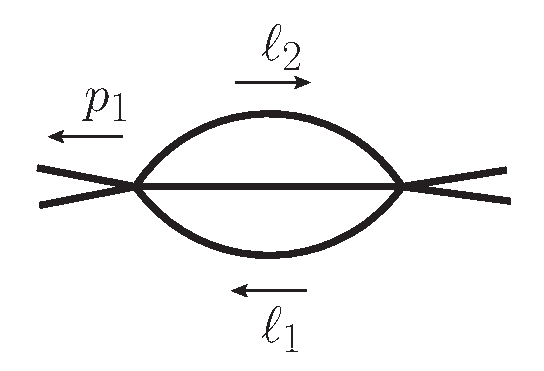
\includegraphics[width=1\linewidth]{sunrise_kinmatics_example}
\end{wrapfigure}
As a two-loop example, we choose a two-loop massless ``sunrise'' topology, which is simple enough to fit the answer on a page.
For $L=2$ we have 11 scalar products. There are 3 propagators in the sunrise, so we have 8 ISPs in total, 
from which 6 are transverse. 
We choose the independent variables to be 
\begin{align*}
  \rho_1 &= \ell_1^2,            \qquad & \alpha_1 = 2 (\sp(\ell_1,p_1)), \\
  \rho_2 &= \ell_2^2,                    & \alpha_2 = 2 (\sp(\ell_2,p_1)), \\
  \rho_3 &= (\ell_1-\ell_2-p_1)^2. &
\end{align*}
Using the formula \cref{eq:number_of_monomials} we get that there are 45 monomials up to the total degree 2.
39 of them contain at least one of the transverse ISPs, so we traceless complete them as in the one-loop case.
We are then left to deal with 6 monomials
\[
  \{1,~ \alpha_1,~ \alpha_2,~\alpha_1^2,~\alpha_1\alpha_2,~\alpha_2^2\}.
\]
Employing the ansatz \eqref{eq:unitarity_compaible_ibp_ansatz} we find lots of unitarity-compatible IBP vectors.
A couple of examples are:
\begin{equation*}
  \begin{tabular}{CC}
    v_1^\mu & v_2^\mu \\
    \midrule
    ( s -\alpha_2)\qty(( s  - \alpha_1) \ell_1^\mu + \rho_1 p_1^\mu)  &   (\alpha_2- s ) \qty( ( s +\alpha_2^2)\ell_2^\mu - \rho_2 p_1^\mu) \\
    (\alpha_1- s )\ell_1^\mu - \rho_1 p_1^\mu         &     ( s +\alpha_2) \ell_2^\mu - \rho_2 p_1^\mu \\
    \left( 2 s  - 2\alpha_1+\alpha_2 \right) \ell_1^\mu + \left( - s +\alpha_1-\alpha_2 + \rho_1 -\rho_2+\rho_3 \right) +\alpha_1\ell_2^\mu &  0\\
    \ldots{} & \ldots{}\\
    %\multicolumn{2}{C}{\ldots{}\ldots{}} \\
  \end{tabular},
\end{equation*}
where $s\coloneqq p_1^2$.
We use all these vectors to obtain the corresponding surface terms. 
In the next step, we find the spanning set.
To do this, we treat each surface term as a vector from the vector space 
$\spn{1,~ \alpha_1,~ \alpha_2,~\alpha_1^2,~\alpha_1\alpha_2,~\alpha_2^2}$,
and find a basis of the subspace spanned by all surface terms. 
It is important that we do this modulo RSPs, i.e.\ (temporarily) set $\rho_j\to 0$.
In this case, we find that 5 of them are independent:\footnote{
  Here we could set all $\rho_i$ to zero, since all integrals below the massless sunrise are scaleless.
  In general, however, it is not the case, so we keep them for illustration.
}
\begin{equation*}
  \small
  \begin{array}{l|l}
    s_1 & \alpha _1^2 (1-D)+\alpha _2^2 (-1+D)+s \left(\rho _1-2 \rho _2+\rho _3\right) \\
    s_2 & \alpha _1^2 (-3 (-1+D) (-4+3 D))+s \left(4 (-1+D)^2 s+3 (-4+3 D) \rho _1-6 (-2+D) \rho _2+3 (-4+3 D) \rho _3\right) \\
    s_3 & \alpha _1^2 ((-1+D) (-3+2 D))+\alpha _2 \alpha _1 \left(2 (-1+D)^2\right)+s \left((3-2 D) \rho _1-2 \rho _2+(3-2 D) \rho _3\right) \\
    s_4 & \alpha _1^2 (-4+(7-3 D) D)+\alpha _1 \left(2 (-1+D)^2 s\right)+s \left((-4+3 D) \rho _1-2 (-2+D) \rho _2+(-4+3 D) \rho _3\right) \\
    s_5 & \alpha _1^2 ((-1+D) (-4+3 D))+\alpha _2 \left(2 (-1+D)^2 s\right)+s \left((4-3 D) \rho _1+2 (-2+D) \rho _2+(4-3 D) \rho _3\right) \\
  \end{array}
\end{equation*}
This leaves us with just one master integral, which
we can choose to be any insertion linearly independent from $\spn{s_1,\ldots{},s_5}$.
For example, it can be the scalar integral.



%\subsection{Factorizable Topologies}

%We construct parametrization as 1-loop squared.
%Thus exactly as in 1-loop we find that all topologies with triangles
%with 1 or 2 external masses do not have masters and the surface term can be taken exactly the same as from 1-loop triangle.
%All other have exactly one master and otherwise the space is spanned by traceless completions.


\section{Cut Equations}
\label{sec:cut_equations}
{

In the previous section, we discussed how to construct a master/surface basis
of all possible numerators for each topology, so the integrand of an amplitude must 
be reducible to the form
\begin{equation} \label{eq:unitarity_ansatz}
  A^{(L)}(\{p_i,\varepsilon_i\}, \{\ell_k\}, D) \longrightarrow  
  \sum_{\Gamma \in \Delta} \sum_{\gamma_\Gamma} \sum_{i \in M_{\Gamma\gamma_\Gamma} \cup S_{\Gamma\gamma_\Gamma}} c_{\Gamma\gamma_\Gamma, i}(\vb*{x},D) \;
  \frac{m_{\Gamma\gamma_\Gamma, i} (\vb*{x},D;\vb*{\rho},\vb*{\alpha}) }%
    {\prod_{j\in P_\Gamma} \rho_j^{\gamma_{\Gamma i, j}}},
\end{equation}
whatever the initial representation of the amplitude on the left-hand side is.
For example, it can be obtained as a sum of all Feynman diagrams.
The only thing left to compute the amplitude is then
to extract the coefficients $c_{\Gamma\gamma_\Gamma, i}$.
In principle, we could sample the expression on the left-hand side with a sufficient number of loop momenta,
and get a linear system of equations for $c_{\Gamma\gamma_\Gamma, i}$ by matching it to our ansatz on the right hand side.
But the system obtained in this way would be so humongous that even a numerical solution would be problematic,
not to mention that evaluating the left hand side is usually not cheap either.

\def\gleading{{\gamma^{\textit{(l)}}_{\Gamma}}}
Fortunately, the insights from generalized unitarity (see \cref{sec:unitarity}) suggest
a physics-motivated way of block-triangularizing the linear system for the coefficients $c_{\Gamma\gamma_\Gamma, i}$.
If we pick a topology $\Gamma$ and arrange loop momenta to satisfy its on-shell limit $\rho_j \to 0,\;\forall j\in P_\Gamma$ (i.e.\ perform a cut),
the coefficients $c_{\Gamma\gleading,i}$ of the leading term in this limit
can be obtained through \textbf{cut equations},
\begin{multline} \label{eq:cut_equations}
  \lim_{\ell^{\phantom{\Gamma}}_l \to \ell_l^{\Gamma}}\qty\Big( A^{(L)} \; {\prod_{j\in P_\Gamma} \rho_j^{\qty(\gleading)_j}} ) =  \\
  %
  \sum_i c_{\Gamma\gleading, i} ~ m_{\Gamma\gleading, i} \quad + \quad 
  %
  \sum_{\Gamma^\prime > \Gamma} \sum_{\gamma_{\Gamma^\prime}, i} 
  c_{\Gamma^\prime\gamma_{\Gamma^\prime}, i} \;
  \frac{m_{\Gamma^\prime\gamma_{\Gamma^\prime}, i}}{\displaystyle \prod_{j\in P_{\Gamma^\prime} \setminus P_\Gamma} \rho_j^{\gamma_{\Gamma^\prime i, j}}},
\end{multline}
which are \cref{eq:unitarity_ansatz} with terms of $\order{\rho_j^{\qty(\gleading)_j}}$ dropped, so
the sum $\sum_{\Gamma^\prime > \Gamma}$ is over topologies with more propagators 
(recall the organization into hierarchies by \cref{eq:topology_order,eq:topology_sequence}).
The cut equations are the core of the numerical unitarity method.
They are formulated for loop momenta $\ell_l^{\Gamma}$ that satisfy the cut conditions,
which we should take into account when choosing sample values to generate the linear systems. 
In this way, going from the top of the hierarchy to the bottom
we solve cut equations one topology at a time, recycling the coefficients obtained earlier, effectively making the initial system block-triangular.

What is even better is that the left-hand side of \cref{eq:cut_equations}, in the on-shell limit,
can be evaluated as products of on-shell tree amplitudes,
\begin{equation} \label{eq:cut_amplitude}
    \lim_{\ell^{\phantom{\Gamma}}_l \to \ell_l^{\Gamma}}\qty\Big( A^{(L)} \; {\prod_{j\in P_\Gamma} \rho_j^{\qty(\gleading)_j}} ) \longrightarrow 
      \sum_{\text{states}} ~ \prod_{i \in T_\Gamma} A^{(0)}_i(\ell_l^{\Gamma},D),
\end{equation}
where the sum is over all states in $D$ dimensions, and $T_\Gamma$ corresponds to
all vertices of the topology $\Gamma$. The fact that this factorization takes place
at the level of the \emph{integrand} is closely related but does not directly follow from generalized unitarity.
In practice the factorization can be rather straightforwardly realized by noticing the following \cite{Eden:1966dnq}: 
if one collects together all Feynman diagrams contributing to a particular topology,
each vertex of this topology is a sum of all tree graphs with fixed external legs,
hence it can be nothing else than a tree amplitude.
For an explicit example of how this happens, see \cref{fig:example_factorization}. 
A notable exception to this observation can be found in the models which
contain non-trivial wave-function and mass renormalization for some of its particles,
i.e.\ when there are non-vanishing one-particle-reducible diagrams \cite{Ellis:2008ir,Ellis:2011cr}.
These Feynman diagrams (see \cref{fig:wbb:singdoublecut}) are absorbed into renormalization and have to be discarded from amplitudes by hand, hence
the vertices of the cut topologies to which they would contribute are \emph{not} tree amplitudes.
There is an interesting proposal to work around this issue \cite{Badger:2017gta}.
In practice, however\footnote{%
  in this thesis we do not aim to follow the philosophy of ``never going off-shell'',
  but rather opt for whichever solution deemed more practical
},
it does not prevent us from using cut equations but rather
demands some additional booking-keeping.

\begin{figure}[ht]
  \[
    \setlength{\figureheight}{0.07\textheight}
    \mathfigure{height=\figureheight}{example_tree_corner/f1} + 
    \mathfigure{height=\figureheight}{example_tree_corner/f2} + 
    \mathfigure{height=\figureheight}{example_tree_corner/f3}+ 
    \mathfigure{height=\figureheight}{example_tree_corner/f4} \longrightarrow 
    \mathfigure{height=1.5\figureheight}{example_tree_corner/corner}
  \]
  \caption{An illustration of diagrammatic verification of factorization. 
    On the left we show all Feynman diagrams contributing to a four-point one-loop amplitude of any theory with 3- and 4-point vertices
    in the channel $\{\ell^2,(\ell-p_1)^2,(\ell-p_1-p_2)^2\}\to 0$ given by the topology on the right.
    The tree amplitudes in the corners of the topology are assembled explicitly.
  } 
  \label{fig:example_factorization}
\end{figure}

Let us now mention how do we handle
the cases when the set of choices of propagators' exponents for some topology $\Gamma$
contains more than one element, that is, there are propagators raised to powers greater than 1 \cite{Abreu:2017idw}.
As we mentioned above, the \cref{eq:cut_equations} directly isolates coefficients of 
the propagator structure with maximal total degree $\gleading$. For this propagator structure
also the factorization of \cref{eq:cut_amplitude} applies.
The coefficients of all the remaining propagator structures can be obtained together with the (leading) coefficients  of a topology one level below
$\Gamma$ in the hierarchy by ``undoing'' the block-triangularization.
Consider an example in \cref{fig:example_subleading_pole}.
The two-loop bubble-hexagon topology $\Gamma_1$ is given by a list of propagators $\{\rho_1,\ldots{},\rho_6\}$ and there are two
possible sets of exponents,
\[
  \Gamma_1 \leftrightarrow  \{\rho_1,\ldots{},\rho_6\}, \qquad \gamma_{\Gamma_1} =  
  \begin{pmatrix} 
    \{1,1,1,2,1,1\} &\leftarrow \gamma_{{\Gamma_1},1}  & \equiv \gamma_{\Gamma_1}^{(\textit{l})} \\ 
    \{1,1,1,1,1,1\} &\leftarrow \gamma_{{\Gamma_1},2} &
  \end{pmatrix}
\]
First, we solve the cut equations for coefficients of $\gamma_{{\Gamma_1},1}$, and proceed down the hierarchy normally until we reach
the bubble-box topology $\Gamma_2$, not considering equations for the coefficients $\gamma_{{\Gamma_1},2}$.
We obtain the latter through the cut equations for $\Gamma_2$, treating them as unknowns together with 
the coefficients of the topology $\Gamma_2$ itself. Clearly, this ``trick'' can always be performed
notwithstanding how many doubled (or tripled, etc.\@) propagators we encounter.
The only cost is that of solving the equations for a larger number of coefficients.

Another possibility is to realize that the only cases when propagators can be raised to higher powers 
are from self-energy insertions on internal lines, which are associated with renormalization.
It turns out \cite{Baumeister:2019rmh} that
it is possible to cook up \emph{integrand-level} UV counter-terms such that
the integrand of the amplitude gets renormalized,
and all subleading poles vanish as a consequence.

We opt for the former approach as a simpler generic solution in favor of the
more intricate case-by-case study of the latter.
We observe that at least for two-loop
amplitudes a slight increase of ranks for some of the cut equations does not
pose any significant problem.

\begin{figure}[ht] 
  \centering
  \begin{tikzpicture}[scale=3,line width=1pt]
    \setlength{\figureheight}{0.08\textheight}
        % Maximal
    \node at (0,2){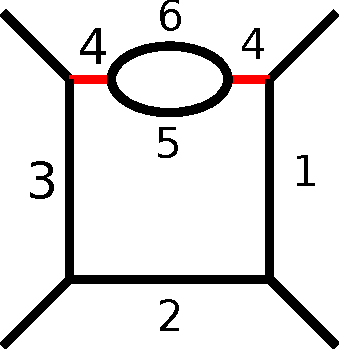
\includegraphics[width=\figureheight]{diagrams_from_4gluon/HexaBubbleThin}};
    \node at (0,1.5){ $\Gamma_1^{\{1,1,1,2,1,1\}}$}; 
    \node at (1,2){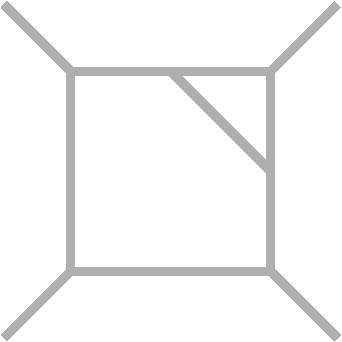
\includegraphics[width=\figureheight]{diagrams_from_4gluon/PentaTriangleThin}};
    \node at (2,2){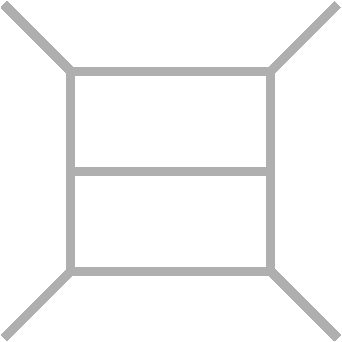
\includegraphics[width=\figureheight]{diagrams_from_4gluon/DoubleBoxThin}};
    \node at (3,2){\reflectbox{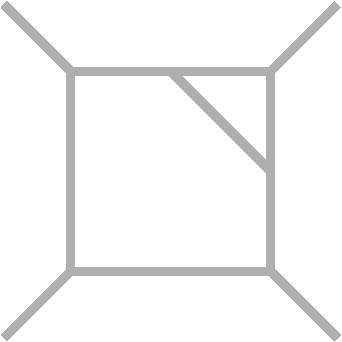
\includegraphics[width=\figureheight]{diagrams_from_4gluon/PentaTriangleThin}}};
        % Next-to-maximal
    \node at (0.5,1) (a) {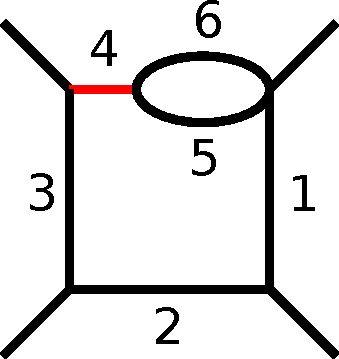
\includegraphics[width=\figureheight]{diagrams_from_4gluon/BubblePentagonSemiGenericThin}};
    \node at (0.5,0.5)  { $\Gamma_1^{\{1,1,1,1,1,1\}}$}; 
    \node at (1.5,1){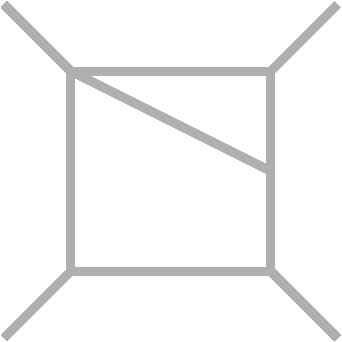
\includegraphics[width=\figureheight]{diagrams_from_4gluon/BoxTriangleThin}}; 
    \node at (2.5,1){\reflectbox{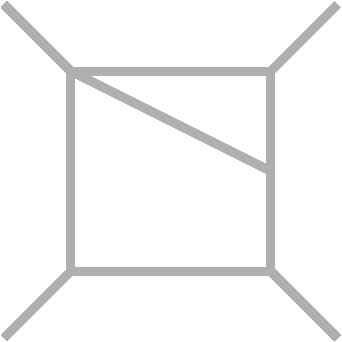
\includegraphics[width=\figureheight]{diagrams_from_4gluon/BoxTriangleThin}}};
        % Next-to-next-to-maximal
    \node at (1.5,0) (b) {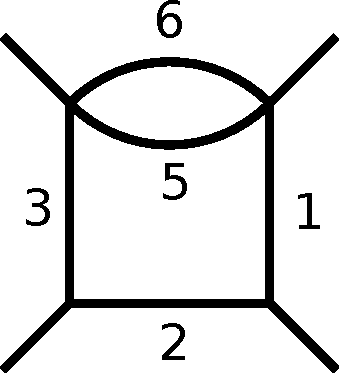
\includegraphics[width=\figureheight]{diagrams_from_4gluon/BubbleBoxGenericThin}};
    \node at (1.5,-0.5){$\Gamma_2^{\{1,1,1,1,1\}}$}; 
    \path [line,<->] (a.south east) -- (b.north west);
  \end{tikzpicture}
%
  \caption{A slice of the hierarchy of a two-loop four-point amplitude with the bubble-box topology $\Gamma_2$ at the bottom.
    The indices $i$ on the lines correspond to the propagators $\rho_i$, and the list of their exponents is given by the superscripts.
    One of the diagrams with topology $\Gamma_1$ has a doubled propagator $\rho_4$.
  }
  \label{fig:example_subleading_pole}
\end{figure}


}

\section{Evaluation of Cuts}
\label{sec:evaluation_of_cuts}

In this section, we discuss the evaluation of the left-hand side of the cut equations \eqref{eq:cut_equations}
in the factorized form of \cref{eq:cut_amplitude}.
For this, we will need to know the explicit components of loop momenta solving the on-shell conditions for each topology.

\subsection{On-Shell Loop Momenta}
\label{sec:osm}

Given any topology $\Gamma$ with $N$ external momenta $\{p_1,\ldots{},p_N\}$, $L$ loops and $N_p$ propagators, our aim
is to find the components of $L$ loop momenta such that  
the cut conditions,
\[
  \rho_j = 0, \quad \forall j\in P_\Gamma,
\]
are satisfied. 
In principle, the equations can be solved case by case given any initial choice of degrees of freedom.
However, we would like the solution to be universal so that we can easily
implement it in a computer program once and for all. 
Furthermore, to be able to use it for both floating-point and exact (finite field) numerical evaluations, 
we would like to avoid non-rational operations as much as possible.
The latter is in general non-trivial since the cut conditions are quadratic, and
define an algebraic variety in a $(D\cdot L)$-dimensional space.
To this end, we closely follow the construction of ``natural'' coordinates described in \cite{Ita:2015tya, Abreu:2017xsl}.

\begin{figure}[ht]
  \centering
  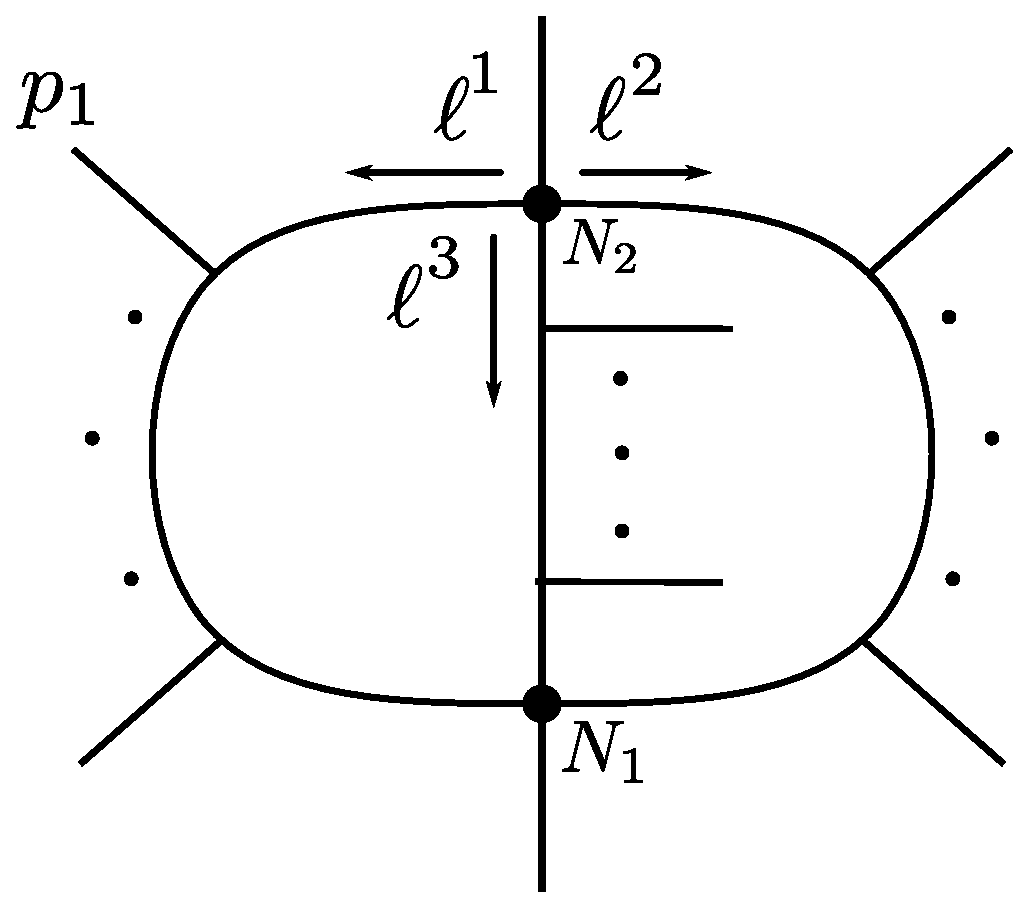
\includegraphics[width=0.3\textwidth]{topo_kinematics}
  \caption{A generic two-loop topology. All external momenta $p_i$ are outgoing. There are 3 strands connecting nodes $N_1$ and $N_2$.}
  \label{fig:topo_kinematics}
\end{figure}

We begin by considering each strand (see \cref{fig:topo_kinematics}) of the topology $\Gamma$ independently.
First, we separate four-dimensional part and $(D-4)$-dimensional parts as
\begin{equation}
  \ell^l = \ell_{[4]}^l + \sum_{i\in \tilde{B}} \tilde{n}_j~\mu^l_{j}, \qquad \sp(\ell^l_{[4]},\tilde{n}) = 0, 
\end{equation}
where $\tilde{n}_i$ is some basis in $\mathsf{S}_{[D-4]}$.
For each strand $l$ we construct a van Neerven-Vermaseren basis (see \cref{sec:vNV_basis})
in $D=4$ with respect to the set $B^l = B^l_p \cup B^l_t$ of $\max(4,N-1)$ external momenta selected in the following order:
\begin{enumerate}
  \item momenta flowing out of strand $l$ (added to $B^l_p$),
  \item any other external momenta until $\max(4,N-1)$ of them is collected (added to $B^l_t$)
\end{enumerate}
Then for $\ell^l_{[4]}$ we get
\begin{subequations}
  \label{eq:lparametrization}
  \begin{align}
    \ell^l_{[4]} &= \sum_{j\in B^l_p} r^l_j(\vb*{\rho}^l)\,v^l_j ~+~ \sum_{j\in B^l_t} \alpha^l_j\,v^l_j ~+~\sum_{j\in B_\tau} \alpha^{\tau l}_j \frac{\tau_j}{(\tau_j)^2}, \\
    \label{eq:lparametrization_b}
    r_j^l(\vb*{\rho}^l) &=  \sp(\ell^l, p_j), \quad j\in B^l_p,    \\ 
    \label{eq:lparametrization_c}
    \alpha_j^l &=  \sp(\ell^l, p_j),\quad j\in B^l_t, \\
    \label{eq:lparametrization_d}
    \alpha_j^\tau &=  \sp(\ell^l, \tau_j),
  \end{align}
\end{subequations}
where $v^l_j$ are dual vectors to $p_j$, and $\tau_j$ are transverse to all external momenta of the topology.
We choose the propagators on the strand $l$, $\vb*{\rho}^l \in P_\Gamma^l \subset P_\Gamma$
as the first set of coordinates for our loop momenta. By construction $\cup_l P_\Gamma^l = P_\Gamma$,
so this trivially matches the choice of variables in \cref{chap:stdtech}.
The momentum conservation constraints from the nodes of the topology will
trivially match $\alpha_j^{\tau l}$ to the transverse ISPs from \cref{sec:ansatz_integrand},
and give \emph{linear} equations between $\alpha_j^l$ which can be used to
relate them to any choice of remaining ISPs $\hat{\vb*{\alpha}}$.
%This way we parametrized $4 L +\frac{1}{2}L(L+1)$ (recall \cref{eq:sps_all}) degrees of freedom from $(D\cdot L)$
%with the scalar products.
This, in fact, provides the lower bound on the dimension $D^{(L)}$ in which we can embed $L$ loop momenta
to be able to reproduce the required number of the scalar products,
\begin{equation}
  D^{(L)}  >  4 +\frac{1}{2}(L+1).
\end{equation}
The equality here cannot be taken except for the case of $L=1$ since we need additional degrees of freedom
(\todo{ask Harald how this can be explained properly from geometry})
for rotations.

What we achieved is that the on-shell conditions are trivialized,
and the only remaining constraints are for the components of $\va{\mu}_j$,
\begin{equation}
  \va{\mu}_i \cdot \va{\mu}_j  \equiv  \mu_{ij} (\vb*{\rho},\vb*{\alpha}) = \ell_i\cdot \ell_j - \ell_{i[4]}\cdot \ell_{j[4]},
\end{equation}
which can be easily solved once and for all.
It is also possible to work around the square roots appearing from these equations (see \cref{sec:muij_square_roots} for details),
so the parametrization can be employed for computations with finite fields.

We conclude this section with two remarks.
\todo{
  In $D$ dimensions we don't have to worry about branches of solutions, 
  and also loop momenta can be real
}
Although in principle the parametrization described in this
section is amenable for both floating-point and exact evaluations,
the former requires the issues of numerical stability to be considered.
And in principle better-suited parametrizations can be derived (see e.g.\ \cite{Kilgore:2007qr,Berger:2008sj} for one-loop examples),
which can be rather tedious already at one loop.

\subsection{Evaluation of Tree Amplitudes}
\label{sec:evaluation_of_tree_amplitudes}

With the on-shell loop-momenta components available
we can evaluate the cuts in \cref{eq:cut_amplitude} as products
of tree amplitudes.

In \cref{eq:unitarity_ansatz} we have constructed  the basis of numerator insertions using Lorentz-invariants, and
the only explicit trace of the dimensional regularization was the presence of rational functions in $D$.
The evaluation of cuts in $D$ dimensions is much more involved since we need to treat the particles' states accordingly.
And a numerical evaluation is only possible if a finite (and preferably) small representation for these states exists.
In \cref{sec:osm} we found that thanks to Lorentz symmetry we can embed loop
momenta into a space with finite integer dimension $D^{(L)}$.
Taking advantage of this fact, we can embed the states of particles in a space of finite integer dimension $D_s\geq D^{(L)}$ as well.
From now on we will keep $D_s$ and $D$ separate,
and only after all master coefficients are determined will we set $D_s\to D\to 4-2\epsilon$.
In \cref{chap:dshel} we examine closely how to deal with the $D_s$-dependence efficiently.
In any case we need to be able to evaluate the tree amplitudes in arbitrary $D_s$ dimensions.

To this end, we choose to utilize the off-shell Berends-Giele recursion \cite{Berends:1987me}
as a very flexible and efficient way to organize tree-level calculations
which admits a seamless generalization to $D_s$ dimensions.
The Berends-Giele recursion is formulated in terms of
\emph{off-shell currents} $J^{\bar{\alpha}}(\{p_i,\alpha^i\})$,
\begin{equation}
  \mathfigure{width=0.2\linewidth}{off-shell_current},
\end{equation}
defined as the sum of all possible ways (using the Feynman rules of the model)
to combine the legs with indices $\{\alpha^1,\ldots{},\alpha^n\}$ and
momenta $\{p_1,\ldots{},p_n\}$ into an open index of type $\bar{\alpha}$.
Here the indices $\alpha$ are understood to refer to tensor or spinor indices, as well as all other relevant quantum numbers such as
charge, flavor, color, etc.
Then starting from the first-level currents, which are simply the external states of particles, one
can recursively (see \cref{fig:BG_recution}) build up the final current
\begin{figure}[!ht]
  \centering
  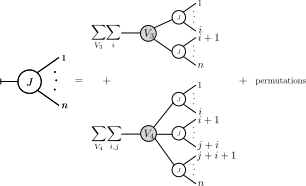
\includegraphics[width=0.8\textwidth]{BG_recursion}
  \caption{A step of the off-shell recursion for a model with 3- and 4-point vertices. All possible permutations of $\{1,\ldots{},n\}$ are considered on the right.}
  \label{fig:BG_recution}
\end{figure}
containing all but one external particle.
The tree amplitude is then obtained by contracting this current with the last remaining external state.
This topic is very well covered in the literature (see e.g.\ \cite{Ellis:2011cr,Weinzierl:2016bus}), so we will refrain from further details.

One of the consequences of unitarity is that the numerators of on-shell propagators are
sums over physical polarization states (in $D_s$ dimensions),
e.g.\ for spin 1 and spin $\frac{1}{2}$ particles
\begin{subequations}
  \begin{align}
    -g^{\mu\nu} + \frac{\ell^\mu \eta^\nu + \ell^\nu \eta^\mu}{\sp(\ell,\eta)}  &~\xleftrightarrow{\ell^2\to 0\;}~  \sum_{j=1}^{D_s-2} \varepsilon^\mu_j(\ell){\varepsilon^\nu_j}^{\star{}}(\ell) , \\
    \qty(\slashed{\ell}  \pm m\,\mathbb{1})^{\alpha\beta} &~\xleftrightarrow{\ell^2\to m^2}~ \sum_{j=1}^{2^{\frac{D_s}{2}-1}} u^\alpha_j(\ell){\overline{u}_j^\beta}(\ell),
  \end{align}
\end{subequations}
so on the cut we are allowed to switch back and forth.
The off-shell recursion provides a very convenient way to take advantage of this fact \cite{Badger:2012pg,Peraro:2016wsq}.
Consider \cref{fig:topo_cut}. Given a choice of a path along the cut,
we decompose into the state sums only the cut propagators at the beginning and at the end of the path.
Moving along the path, 
for each tree amplitude we build its final current,
but instead of contracting it with the external state, we feed it through
the corresponding cut propagator as an input to the next tree amplitude.
Only at the end of the path do we contract the final current with a state from a polarization sum.
Note that beyond two loops it is not always possible to span the whole cut with just one continuous path.

\begin{figure}[ht]
  \centering
  \subfloat[\label{fig:topo_cut:path}]{
    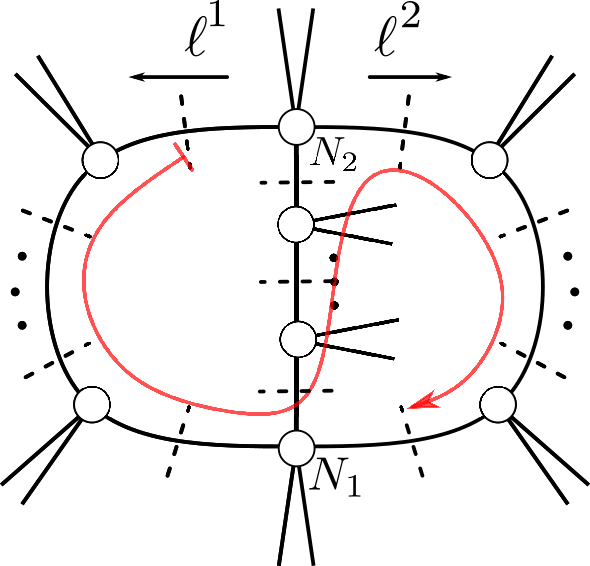
\includegraphics[width=0.3\textwidth]{topo_cut}
  }
  \hfill
  \subfloat[\label{fig:topo_cut:unrolled}]{
    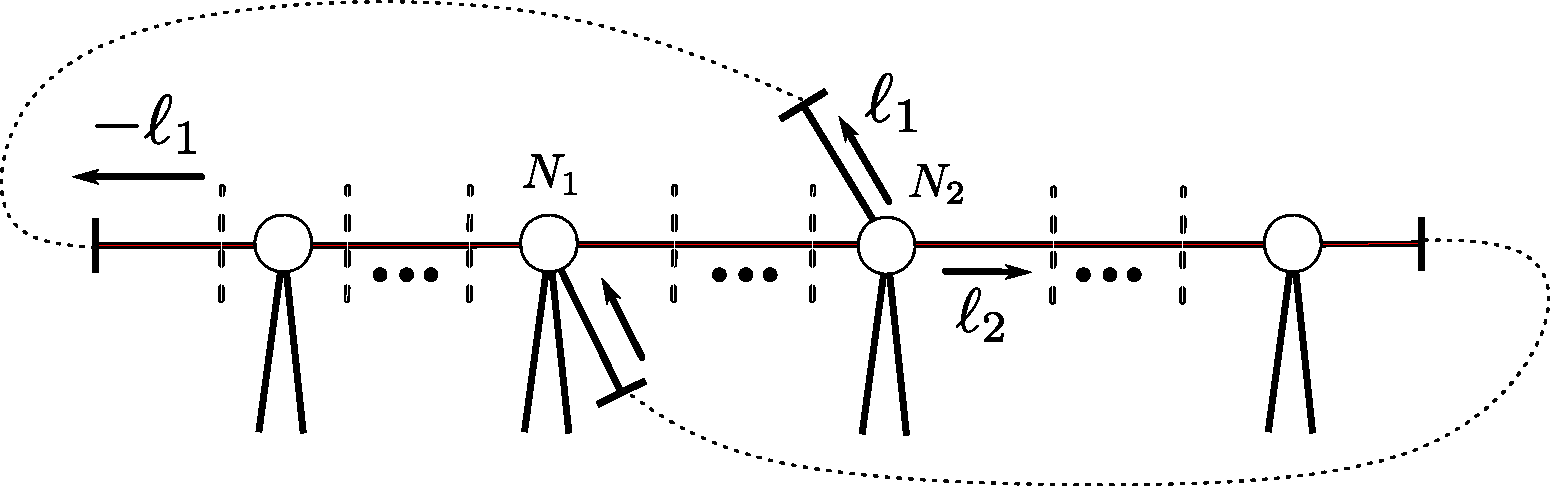
\includegraphics[width=0.6\textwidth]{topo_unrolled}
  }
  \caption{A generic cut of a two-loop amplitude as a sequence of ``closed'' off-shell currents, shown as blobs.
    The red line in \cref{fig:topo_cut:path} demonstrates a path, which is ``unrolled'' in \cref{fig:topo_cut:unrolled}.
    The dashed lines in \cref{fig:topo_cut:unrolled} indicate the only two cut propagators
    decomposed into pairs of polarization states and used as an explicit input to the off-shell recursion.
  }
  \label{fig:topo_cut}
\end{figure}

\todo{Gauge invariance is explicit in on-shell quantities, so no need to include ghosts.} 

\subsection{Dimensional Reconstruction}
\label{sec:dimensional_reconstruction}

We now have everything required to obtain the coefficients of master integrals 
$c_{\Gamma\gamma_\Gamma,i}$ from  \cref{eq:cut_equations}.  
The coefficients are functions of external kinematics $\vb*{x}$, and the dimensional regularization parameters $D$ and $D_s$.
In the spirit of our goal of constructing a fully numerically-capable framework, 
we can obtain the master coefficients
for any numerical value of $D$\footnote{
  here $D$ refers exactly to the parameter in the master/surface decomposition,
  and  not to be confused with the dimensionality of the space in which we embed loop momenta
}%
\textsuperscript{,}%
\footnote{as long as we avoid explicit poles on integer values},
and any  \emph{integer} value of $D_s$ large enough to embed the loop momenta components.
The internal self-consistency of dimensional regularization guarantees
that these evaluations reproduce correctly the corresponding limits from the formally infinite-dimensional spaces.\footnote{
  Beware of models with chiral couplings! A naive ``continuation'' of chirality to $D_s$ dimensions
  can make all coefficients to behave non-smoothly as functions of $D_s$ at all integer values.
}

We do however need to know the full analytic dependence on both $D$ and $D_s$ to be able
to set them to $4-2\epsilon$ eventually.
To this end, we employ the function interpolation techniques (see \cref{sec:func_reconstruction})
and reconstruct the rational dependence on $D$ and polynomial dependence on $D_s$ for each coefficient from numerical samples.
This idea is known by the name of
\emph{dimensional reconstruction} \cite{Giele:2008ve,Ellis:2008ir,Boughezal:2011br,Abreu:2017xsl,Abreu:2017hqn}.
In some cases evaluating the left hand side of \cref{eq:cut_equations} for multiple $D_s$ values might become a computational bottleneck,
for example when fermionic particles appear in loops. In \cref{chap:dshel} we discuss how to address this issue.

We conclude this section with some technical remarks which
have important implications for numerical efficiency of the dimensional reconstruction.
\begin{itemize}
  \item Since the master integral coefficients depend both on $D$ and  $D_s$ at a first glance we would
    need to evaluate everything $n_D \cdot n_{D_s}$ times, where $n_D$ and $n_{D_s}$ are the sizes of the respective samples.
    However since the $D$-dependence comes solely from the right hand side of \cref{eq:unitarity_ansatz}
   and the $D_s$-dependence from the left hand side, we can sample each side independently only $n_D$ and $n_{D_s}$ times
   accordingly.
 \item Although we do need to determine the surface-term coefficients from \cref{eq:cut_equations} to use them for subtractions,
   we \textit{do not} need to reconstruct their dependence on $D$ analytically. 
   This is very helpful because the surface-term coefficients can be expected to be more complicated in general
   since they do not contain physical information and ambiguous to a great extent.
   %This is the first example of how numerical evaluations avoid the complexity of large intermediate expressions,
   %but the analytic result is obtained in still.
 \item The reconstruction algorithms normally work with exact numerical evaluations only.
   However even if we aim for example for Monte-Carlo integration over external phase space using floating point numbers,
   the rational functions of $D$ can be reconstructed for each process from just one exact ``warm-up'' evaluation over finite fields.
\end{itemize}

\section{Discussion}
In this chapter we laid out the central concepts of the multi-loop $D$-dimensional numerical unitarity approach.
We formulated it in a way directly amenable for automation.
And indeed we implemented the presented algorithms to obtain the results of \cref{chap:5parton}.

The major ingredients of our method, 
the master/surface integrand parametrization and
the usage of generalized cuts to obtain cut equations
are largely independent of each other and in fact 
can be used separately if deemed beneficial.

The cut equations can be employed to obtain the coefficients of any basis of integrand functions. 
For example, one can consider a basis of simple monomials in \cref{eq:rsp_reduction}.
In this way only the reduction of RSPs will be achieved, and the full IBP reduction has to be preformed afterwards.
One advantage is that the coefficients in this basis do not depend on $D$ (they still depend on $D_s$ of course).
Or one can consider the basis of simple monomials but with transverse ISPs traceless-completed (see \cref{sec:traceless_completion}),
This was analyzed in \cite{Mastrolia:2016dhn}.
In this way, only the IBP reduction of non-transverse ISPs remains to be carried out.
The latter \textit{is} frequently the hardest part of the reduction of multi-loop amplitudes. 
So the fact that the master/surface basis mitigates significantly it's difficulty is the main argument for our choice.

It is also worth mentioning that the evaluation of cuts through the 
factorization property of \cref{eq:cut_amplitude} is not essential in our approach. 
The left hand side of \cref{eq:cut_equations} can in principle be any 
expression which has a form of \cref{eq:general_amplitude} which can be evaluated in the on-shell limit,
like a single Feynman diagram or a numerator insertion on a particular topology. 

%We usead cutting a lot.
%In our approach we made use of cutting in many places.
%``Unitarity'' approaches sometimes simply means anything employing cuts.

%Given the consideration above,

%On the opposite side the master/surface basis and do the full reduction in place.
